\chapter{Diskussion \& Evaluation}
\label{chap:disc_eval}
\label{chap:discussion}
\label{chap:evaluation}

In diesem Kapitel wird das System \name mit allen Komponenten diskutiert und 
evaluiert.
Dabei wird u.\,a. herausgestellt, inwiefern sich \name von den verwandten 
Arbeiten abgrenzt, wie die Webanwendung und die App angelaufen und wie die 
Tester*innen damit zurecht gekommen sind.

\section{Diskussion}
\label{sec:discussion}

Im Gegensatz zu den verwandten Arbeiten bietet \name zu jedem Produkt und jeder 
Zutat eine Veganität an, die in beiden Fällen mit Quellen wie Produktanfragen 
oder Links zu Websites belegt werden können. Insbesondere wichtig dabei ist der 
Kontakt zu den Hersteller*innen, die diese Produktanfragen beantworten können, 
indem zu jedem*jeder Hersteller*in das Hinzufügen von Kontaktdaten möglich 
ist.\\
Jedoch bietet \name im Moment keine weiteren Daten zu einem Produkt an, die für 
eine Kaufentscheidung nützlich wären, wie das z.\,B. bei barcoo der Fall ist.
Wünschenswert wären dazu die Einbindung von folgenden Diensten bzw. Funktionen:
\begin{itemize}
  \item Preisvergleiche, die auch die Geschäfte mit einbeziehen
  \item Bewertungen, z.\,B. im Hinblick auf Geschmack oder 
Preis-Leistungs-Verhältnis
  \item Testergebnisse, z.\,B. von Stiftung Warentest
  \item Ökoinformationen, z.\,B. von Greenpeace, die die Ökobilanz der 
Hersteller*innen aufzeigen
  \item Gesundheitsinformationen, z.\,B. ob ein Produkt hormonell wirksame 
Chemikalien beinhaltet, die von den Verbraucher*innenzentralen oder anderen 
Dienstleister*innen eingebunden werden können
  \item Essenstagebuch, basierend auf den Nährwertangaben, mit dem z.\,B. der 
Tagesbedarf an verschiedenen Nährstoffen kontrolliert werden kann
  \item Ortssuche lokal und global, d.\,h. lokal, in welchem Regal in 
diesem Geschäft und global in welchem Geschäft in 
welcher Stadt sich das gesuchte Produkt oder eine Alternative dazu befindet
\end{itemize}
Diese Modifikationen führen dazu, dass im Endeffekt ein Portal aufgebaut 
wird mit vielen unterschiedlichen Informationen, die für die Verbraucher*innen 
nützlich sein können. Mit dem Unterschied zu den verwandten Arbeiten, dass auch 
Minderheiten wie z.\,B. Rohköstler*innen oder Frutarier*innen beachtet werden 
können und die Daten alle lizenzfrei vorliegen.

Bisher liegen noch keine Daten zu Non-Food Produkten vor, also z.\,B. Kosmetika 
oder Bauteile für Automobile. Die entsprechenden Kategorien sind zwar in \name 
vorhanden, allerdings fehlen die Eingabemöglichkeiten, die bei manchen Produkten 
notwendig sind, z.\,B. die Seitenanzahl bei einem Buch.
Im Zuge dessen könnten auch die Basiszutaten ausgeweitet werden, sodass 
z.\,B. alle E-Nummern vertreten sind und auch chemische oder pharmazeutische 
Namen benutzt werden können.

\name ist im Moment eine Plattform, die sich explizit an Veganer*innen wendet. 
Dies könnte auch im Stil von \ac{MENSSANA} ausgeweitet werden, in dem z.\,B. in 
den Nutzer*inneneinstellungen ein Profil angelegt werden kann, welche Allergene 
oder Unverträglichkeiten vorliegen, um so noch näher bestimmen zu können, 
welche Produkte für die Nutzer*innen geeignet sind.

Wie in Abschnitt~\ref{sec:implementation:veganity} beschrieben, ist die 
Laufzeit bei einem Update der Veganität recht hoch, dies könnte durch 
entsprechende Modifikationen der Algorithmen optimiert werden. Ebenfalls könnten 
die SQL-Abfragen an die Datenbank optimiert werden, indem z.\,B. die Abfragen 
mit "`Join"' zusammengefasst werden.

Auch die Gamifikation, die von \name benutzt wird und bisher die Elemente 
Punkte, Fortschrittsanzeigen und Bestenliste beinhaltet, könnte ausgebaut 
werden (vgl. Abschnitt~\ref{sec:concept:gamification}). So kann sich z.\,B. an 
Websites orientiert werden, die sehr stark auf Gamifikation setzen und für sehr 
viele Aktionen Punkte vergeben oder auf sogenannte Badges, also Abzeichen 
setzen. Zudem könnten nicht nur bei den Produkten, sondern auch bei den Zutaten 
und Hersteller*innen Fortschrittsanzeigen benutzt werden.
Eine gute Umsetzung der Gamifikation findet sich z.\,B. bei den Lernplattformen 
"`Memrise"' und "`Duolingo"', sowie der Frage\,\&\,Antwort-Plattform 
"`Stack Exchange"' \citeweb{memrise, duolingo, stackexchange}.

Um Missbrauch bei der Nutzung von \name vorzubeugen wurden verschiedene 
Maßnahmen ergriffen wie z.\,B. die Validierung der E-Mailadresse und das 
Rechtesystem. In Überlegung war ebenfalls, bei bestimmten Aktionen zu 
bestätigen, dass diese nicht automatisch durchgeführt wird, indem ein Captcha 
eingegeben werden muss. Diese Idee wurde allerdings zu Gunsten der 
Barrierefreiheit verworfen. Stattdessen gibt es nun eine jeweilige Wartezeit von 
10 Sekunden zwischen der Eintragung eines Produktes, einem Kommentar und einer 
Produktanfrage. Allerdings könnte dies noch erweitert werden, indem z.\,B. wie 
bei dem schon erwähnten System Stack Exchange unangebrachte Angaben oder Spam 
durch eine Markierung bei den Administrator*innen gemeldet werden.

Bisher ist \name ein System, das bei einem Update einer Eintragung die alten 
Werte "`vergisst"'. Dies ist insbesondere nicht erwünscht bei wichtigen 
Basiszutaten wie Wasser. Würde bei Wasser nun die Veganität auf unvegan 
geändert werden, müssten auch sehr viele Produkte geändert werden, die dann 
ebenfalls unvegan wären. Dabei müssten dann bei all diesen Produkten z.\,B. 
durch einen Kommentar oder eine Produktanfrage bestätigt werden, dass dies 
immer noch z.\,B. vegan ist.
Von daher sollte ein selbstheilendes System eingebaut werden, dass diese 
Updates registriert und dementsprechend handelt, sodass z.\,B. Produktanfragen 
automatisch generiert und versendet werden.

Die Bedienoberfläche könnte funktionell verbessert werden, indem z.\,B. gerade 
nicht erwünschte Elemente ein- oder ausgeklappt werden können oder in den 
Übersichten nach Einträgen gesucht werden kann oder die Einträge anders 
geordnet werden können. Für \ac{RoR} existieren bereits solche 
Funktionalitäten, allerdings wurde dies bisher nicht implementiert.

Die mobile App benötigt im Moment zum Funktionieren eine Internetverbindung, um 
auf die Datenbank von \name zugreifen zu können. Da aber nicht in jedem 
Supermarkt eine ausreichende Internetverbindung vorliegt, wäre es sinnvoll, 
Daten wie \ac{GTIN}, Name und Veganität der Datenbank lokal auf dem mobilen 
Gerät zu speichern und bei einer besseren Verbindung ggf. zu aktualisieren, die 
dann bei einem Produktscan genutzt werden können.

Weitere Erweiterungen, die zu einer Verbesserung von \name führen können und 
dabei eigene wissenschaftliche Arbeiten bilden, werden in 
Abschnitt~\ref{sec:future_work} beschrieben.

\clearpage
\section{Evaluation}
\label{sec:evaluation}

Innerhalb der einmonatigen Testphase von \name im August 2013 haben sich 14 
Personen über die Anbieter*innen Facebook, GitHub, 
Google und Twitter angemeldet, die
dabei teilweise Daten in das System eingespeist haben.
Werbung für \name wurde nur auf Facebook gemacht, da dort mit über 100 
potentiellen Tester*innen die Reichweite am größten war.
Die Verteilung der Tester*innen auf die Anbieter*innen ist in
Abbildung~\ref{img:users-p-v} dargestellt.

\begin{figure}[ht]
  \centering
  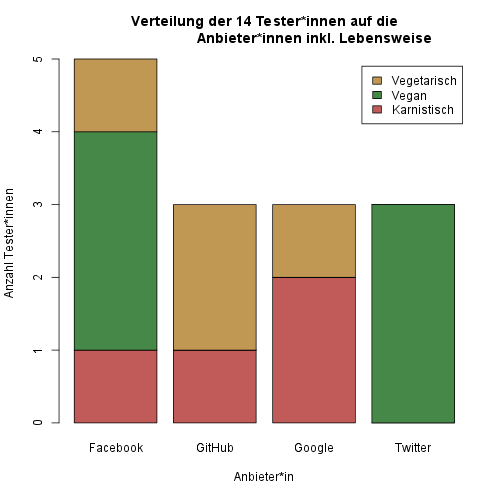
\includegraphics[scale=0.6]{misc/r/users-p-v.png}
  \caption{Verteilung der Tester*innen auf die Anbieter*innen inkl. 
Lebensweisen}
  \label{img:users-p-v}
\end{figure}

Dabei wurde auch die Lebensweise der 
Tester*innen mit einbezogen, in diesem Falle Vegetarisch, Vegan und 
Karnistisch, also einer Lebensweise, die eine Tötung von Tieren nicht 
ausschließt.\\
Die Tester*innen haben insgesamt 111 Produkte angelegt, wobei durch die 
Produkterstellung automatisch 430 Zutaten angelegt wurden. Allerdings waren 
einige Zutaten doppelt, z.\,B. durch falsche Schreibweise oder Zutaten, die 
weitere Zutaten beinhalten wie "`Tofu"' oder "`Teig"', sodass diese 
"`versteckt"' und damit 393 "`echte"' Zutaten kreiert wurden (vgl. 
Abschnitt~\ref{sec:implementation:ingredients}).
Die Produkte und die Verteilung auf die vier Veganitäten ist in 
Abbildung~\ref{img:products} zu sehen, die Verteilung der Zutaten auf die 
Veganitäten in Abbildung~\ref{img:ingredients}.

\begin{figure}[ht]
	\begin{adjustwidth}{-1in}{-1in}
	\centering
	\begin{subfigure}[b]{0.6\textwidth}
		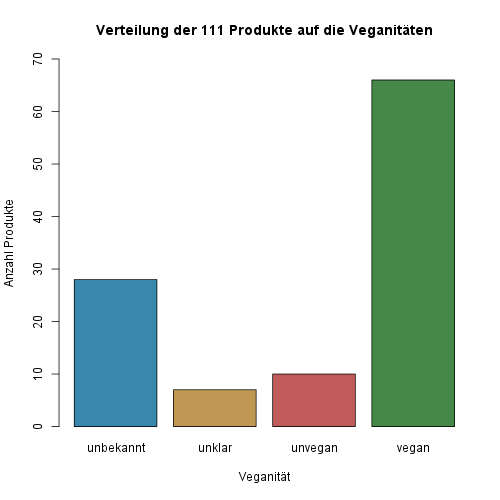
\includegraphics[width=\textwidth]{misc/r/products.png}
		\caption{Verteilung der Produkte auf die Veganitäten}
		\label{img:products}
	\end{subfigure}
	~
	\begin{subfigure}[b]{0.6\textwidth}
		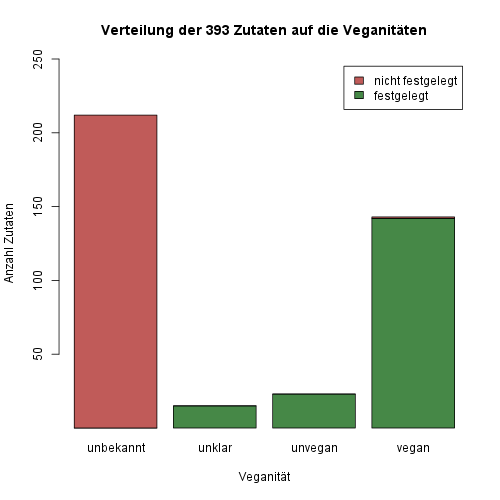
\includegraphics[width=\textwidth]{misc/r/ingredients-f.png}
		\caption{Verteilung der Zutaten auf die Veganitäten}
		\label{img:ingredients}
	\end{subfigure}
	\end{adjustwidth}
	\caption{Diagramme mit verschiedenen Verteilungen auf die Veganitäten} 
	\label{img:evaluation-1}
\end{figure}

Bei den Zutaten wurde noch mit einbezogen, ob 
die Veganität der Zutat von den Administrator*innen festgelegt wurde oder 
nicht, was im Diagramm grün bzw. rot dargestellt ist (vgl. 
Abschnitt~\ref{sec:implementation:ingredients}). Die hohe Anzahl der von den 
Administrator*innen festgelegten Zutaten-Veganitäten ergibt sich daraus, dass 
sehr viele Basiszutaten wie Gewürze, Kräuter, Obst, Gemüse usw. als Produkte 
fehlen und daher schlecht die Produkt-Veganität aus den Zutaten ermittelt werden 
kann. Lediglich die Zutat "`Meersalz"' konnte durch ein Produkt repräsentiert 
werden.
Aus der roten Säule bei "`unbekannt"' kann abgelesen werden, dass über 200 
Zutaten nicht auf Veganität überprüft wurden und standardmäßig nicht 
festgelegt sind.
Insgesamt bieten die jetzt vorhandenen Zutaten eine solide Grundlage, um 
aus der Zutatenliste eines neuen Produktes die Zutaten-Veganität zu berechnen.

Die Qualität bzw. die Vollständigkeit der Produktangaben war -- wie durch die 
Gamifikation erwartet -- hoch, was in Abbildung~\ref{img:integrity-2} deutlich 
wird. Mehr als 75 der 111 Produkte waren fast oder vollständig eingetragen, nur 
zwei Produkte hatten einen Vollständigkeitswert von unter 66\,\%.
Die hohe Qualität der Eingaben zeigt sich auch bei den Häufigkeiten der 
Zutatenanzahlen in einem Produkt, was auf 
Abbildung~\ref{img:products_ingredients} zu sehen ist, da zu jedem der 111 
Produkte Zutaten eingetragen wurden. Dabei haben die Mehrzahl der Produkte 
(nämlich 23) nur eine Zutat, während nur eine kleine Menge von Produkten mehr 
als 20 Zutaten haben. Die meisten Zutaten (nämlich 36) hat genau ein Produkt.

\begin{figure}[ht]
	\begin{adjustwidth}{-1in}{-1in}
	\centering
	\begin{subfigure}[b]{0.6\textwidth}
		
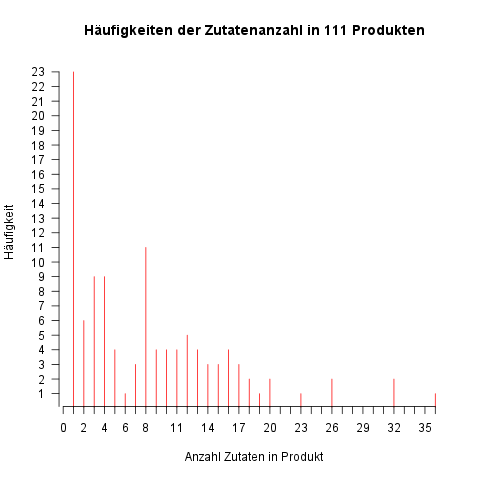
\includegraphics[width=\textwidth]{misc/r/products_ingredients.png}
		\caption{Häufigkeiten der Zutatenanzahl in einem Produkt}
		\label{img:products_ingredients}
	\end{subfigure}
	~
	\begin{subfigure}[b]{0.6\textwidth}
		
\includegraphics[width=\textwidth]{misc/r/integrity.png}
		\caption{Verteilung der Vollständigkeit der Produktangaben}
		\label{img:integrity-2}
	\end{subfigure}
	\end{adjustwidth}
	\caption{Häufigkeiten der Zutatenanzahl in einem Produkt und Verteilung 
der Vollständigkeit der Produktangaben}
	\label{img:evaluation-2}
\end{figure}

Durch die intensive Nutzung der 
Webanwendung und der mobilen App konnten die Tester*innen wertvolles Feedback 
liefern, was zur Verbesserung von \name beigetragen hat.\\
So wurde die Bedienoberfläche durchweg positiv aufgenommen und konnte auch 
von technisch nicht versierten Menschen intuitiv benutzt werden, allerdings 
wurde angeregt, gerade bei Elementen der Gamifikation (vgl. 
Abschnitt~\ref{sec:concept:gamification}) wie dem Punktsystem und der 
Fortschrittsanzeige Hinweise anzuzeigen, wie sich diese auswirken und was sie 
bedeuten.\\
Ebenso konnte
durch die Eintragung von verschiedenen Produkten der
Zutatenparser ständig verbessert und erweitert werden.
Einige Anmerkungen haben zu Datenbankmodifikationen geführt, so 
wurden z.\,B. bei den Zutaten Klassennamen wie "`Konservierungsmittel"' und 
"`Farbstabilisator"' eingeführt, die eine Zutat näher spezifizieren können.
Zudem konnten durch die Nutzung viele Fehler gefunden und beseitigt werden.

Die Funktionalität, die von Anfang an gewünscht war, nämlich durch einen 
Barcode zu erkennen, ob ein Produkt vegan ist oder nicht, wurde durch die 
mobile Anwendung erleichtert und auch im realen Einsatz erfolgreich 
getestet. Verwendet wurden dabei Geräte mit Android ab Version 4.0.
Trotz teilweise geringer Empfangsstärke konnte durch die kleine Menge an Daten, 
die von der App zur Datenbank und wieder zurück gesendet werden, schnell und 
einfach ein Produkt im Hinblick auf die Veganität und damit den Genuß getestet 
werden.
Es wurde bei der App lediglich angemerkt, dass die Veganität besser 
herausgestellt werden sollte wie es z.\,B. bei der verwandten Arbeit 
\ac{MENSSANA} in Abschnitt~\ref{sec:menssana} der Fall ist und die App damit 
als Allergiewarner -- nur mit ethischem Hintergrund -- fungieren soll.